\documentclass[main.tex]{subfiles}
\begin{document}
\section{Introduction}

\emph{Beaucoup de blabla. Beaucoup.}

À part la radio, toute les transmissions sont numériques.
\paragraph{Objectif}
Transmettre le max de donnée avec un fiabilité maximale
\begin{itemize}
\item Malgré les limites théoriques
\item Les contraintes physiques
\item contraintes numériques
\end{itemize}

\section{Historique}
\emph{encore du blabla. encore. }
\section{Principe d'une chaine de transmission numérique}

\begin{figure}[H]
  \centering
  \begin{tikzpicture}
    [every node/.style={draw,rectangle,minimum height=4em,node
      distance=0.5cm,scale=0.8,inner sep=2pt}]
    \node (S) at (0,0){Source};
    \node (CS)   [right= of S]{\begin{tabular}{c}Codage \\ source\end{tabular}};
    \node (CC)   [right= of CS]{\begin{tabular}{c}Codage \\ canal\end{tabular}};
    \node (CBB)  [right= of CC]{\begin{tabular}{c}Codage B de B\\ modulation\end{tabular}};
    \node (C)    [right= of CBB]{Canal};
    \node (A)    [right= of C][adder]{};
    \node (Demod)[right= of A]{Demod};
    \node (E)    [right= of Demod]{Egaliseur};
    \node (Decod)[right= of E]{Decodeur};
    \tikzset{every node/.style={}}
    \draw (S) -- (CS) -- (CC) -- (CBB)-- (C) -- (A.1) (A.3) -- (Demod) -- (E) -- (Decod);
    \draw[latex-] (A.4) -- ++(0,1) node[above]{Bruit};
    \draw [thick,decoration={
        brace,
        mirror,
        raise=0.5cm,amplitude=0.5cm},decorate] (S.south west) -- (CBB.south east)node[midway,below=1cm]{Emetteur};
      \draw [thick,decoration={
        brace,
        mirror,
        raise=0.5cm,amplitude=0.5cm},decorate] (C.south west) -- ++(2.5,0) node[midway,below=1cm]{Canal de transmission};
      \draw [thick,decoration={
        brace,
        mirror,
        raise=0.5cm,amplitude=0.5cm},decorate] (Demod.south west) -- (Decod.south east) node[midway,below=1cm]{Recepteur};
  \end{tikzpicture}
  \caption{Principe d'une chaine de transmission numérique}
\end{figure}

\paragraph{Source}
Une source d'information est un signal aléatoire. Les communications numériques sont alors des signaux discrets.
\paragraph{Codage de source}
Dans cette étape on associe un code de facon bijective une suite de k élement binaire (cf UE 455) $\{c_k\}$
\paragraph{Codage Canal}
L'objectif est de lutté contre les effets du canal:
\begin{itemize}
\item introduction de redondance
\item Ajoute des bits de redondances à $\{c_k\}$ pour former $\{d_n\}$
\item permet l'évaluation d'erreur
\end{itemize}
Il faut trouver un compromis entre débit et robustesse aux erreurs.
\paragraph{Codage de bande de base}
\begin{itemize}
\item Donne une réalité physique au message (tension, énergie...)
\item Utilise des formes d'impulsions
\item Donne au spectre des des propriété utiles (bandes occupée, présence de la fréquence d'horloge ...)
\end{itemize}

\begin{figure}[H]
  \centering
  \begin{subfigure}{0.5\textwidth}
    \centering
    \begin{tikzpicture}
      \begin{axis}
       [axis lines = middle,
        xmin = -0.1,xmax =5,ymin=-0.1,ymax=3,
        xlabel = $t$,ylabel=$g(t)$,xtick={4},xticklabels={$T_b$},
        ytick={2},yticklabels={$V$}]
        \addplot[black,thick] coordinates {(0,2) (4,2) (4,0)};
      \end{axis}
    \end{tikzpicture}
    \caption{impulsion rectangulaire}
    \label{fig:label}
  \end{subfigure}%
  \begin{subfigure}{0.5\textwidth}
    \centering
    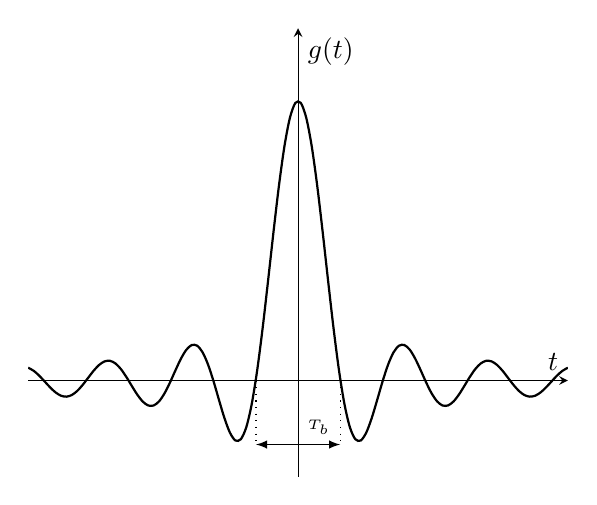
\begin{tikzpicture}
      \begin{axis}
       [axis lines = middle,
        ymin=-0.3,ymax=1.1,
        xlabel = $t$,ylabel=$g(t)$,xtick=\empty,ytick=\empty]
        \addplot[black,thick,smooth,samples=100]
        {50*sin(deg(x*4))/deg(x*4)};
        \draw[latex-latex] (axis cs:-0.78,-0.2) -- (axis cs:0.78,-0.2)
        node[midway, above right]{\tiny$T_b$};
        \draw[dotted] (axis cs: -0.78,0) --(axis cs:-0.78,-0.2)
        (axis cs: 0.78,0) --(axis cs:0.78,-0.2);
      \end{axis}
    \end{tikzpicture}
    \caption{impulsion de Nyquist}
    \label{fig:label}
  \end{subfigure}
  \caption{forme d'impulsion usuelles}
\end{figure}

  \paragraph{Modulation}
  Comme pour une modulation numérique
  \[
    e(t) = A(t)\cos(\Phi(t))
  \]
Où $A(t)$ et $\Phi(t)$ sont les amplitudes et phases instantanée.

\begin{exemple}[Modulation QPSK]
  \begin{figure}[H]
    \centering
    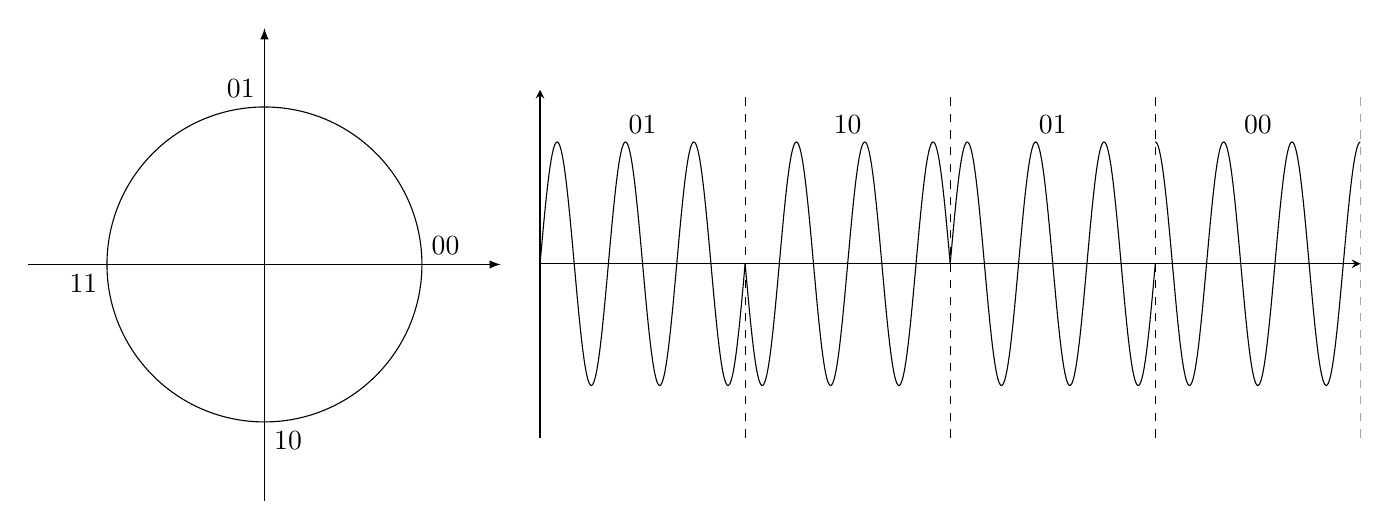
\begin{tikzpicture}
      \begin{scope}
        \draw[-latex] (0,-3) -- (0,3);
        \draw[-latex] (-3,0) -- (3,0);
        \draw (0,0) circle (2);
        \node[above right] at (2,0) {00};
        \node[above left] at (0,2) {01};
        \node[below left] at (-2,0) {11};
        \node[below right] at (0,-2) {10};
      \end{scope}
      \begin{scope}[shift={(3.5,-2.2)}]
        \begin{axis}
          [axis lines = middle,height=6cm, width=12cm,
          xmin=0,xmax=360,ymin=-1,ymax=1,
          domain=0:360,samples=200, xtick=\empty,ytick=\empty]
          \addplot[black,domain=0:90]{0.7*sin(12*x)};
          \addplot[black,domain=90:180]{-0.7*sin(12*x)};
          \addplot[black,domain=180:270]{0.7*sin(12*x)};
          \addplot[black,domain=270:360]{0.7*cos(12*x)};
          \draw[dashed] (axis cs:90,-1) -- (axis cs: 90,1);
          \draw[dashed] (axis cs:180,-1) -- (axis cs: 180,1);
          \draw[dashed] (axis cs:270,-1) -- (axis cs: 270,1);
          \draw[dashed] (axis cs:360,-1) -- (axis cs: 360,1);
          \node at (axis cs: 45,0.8){01};
          \node at (axis cs: 135,0.8){10};
          \node at (axis cs: 225,0.8){01};
          \node at (axis cs: 315,0.8){00};
        \end{axis}
      \end{scope}
    \end{tikzpicture}
    \caption{modulation QPSK}
  \end{figure}
\end{exemple}

\paragraph{Canal de transmission}
Plusieurs types de canaux possibles: canal hertzien , ligne filaire , coax...
On les caractérise par leur réponse impulsionnelle complexe, et par sa bande passante B.
\begin{defin}
  On défini la \emph{ capacité de Shannon:}
  \[
    C = B.\log_2(1+RSB)
  \]
\end{defin}
\paragraph{Bruit}
Le bruit est présent à la transmission, et dans le canal. on le caractérise par sa densité de probabilité généralement on suppose le bruit additif Blanc et Gaussien:

\[
  p(b) = \frac{1}{\sqrt{2\pi \sigma_B^2}} \exp\left(\frac{-(b-\mu_b)^2}{2\sigma_b^2}\right)
\]
On a souvent un bruit centré : $\mu_b=0$

\paragraph{Démodulation}
À la réception on inverse la modulation
\begin{exemple}[Démodulation QPSK]

\end{exemple}
\paragraph{Egaliseur régénerateur}
Objectif : lutter les effets du canal de transmission pour augmenter le débit.

\paragraph{Décodeur}
on refait le passage analogique-numérique et on décode le canal (correction d'erreur) pour cela :
\begin{itemize}
\item echantillonnage (cad prise de décision) :filtrage adapté + sortie dur ou souple
\item décodage du canal
\item décodage de source
\end{itemize}
\end{document}
%%% Local Variables:
%%% mode: latex
%%% TeX-master: "main"
%%% End:
